\documentclass[fleqn]{article}
\usepackage{tikz,tcolorbox}
\usepackage{array} % For customizing tables
\usepackage{booktabs} % For better horizontal lines
\usepackage[a4paper, paperwidth=25cm, paperheight=25.5cm, left=2cm, right=2cm, top=2cm, bottom=2cm]{geometry}
\usepackage{multicol}
\usepackage{amsmath}
\usepackage{pgfplots}

\usepackage[utf8]{inputenc}

\usepackage{listings}
\usepackage{xcolor}


\lstdefinestyle{pythonstyle}{
    language=python,                    % Language set to Python
    basicstyle=\ttfamily\footnotesize,   % Change basic font size
    keywordstyle=\color{blue}\bfseries, % Different keyword style
    stringstyle=\color{red},         % Different string color
    commentstyle=\color{green!60!black}\itshape, % Adjust comment color
    numbers=left,                       % Line numbers on the left
    numberstyle=\tiny\color{gray},      % Smaller number font and color
    stepnumber=1,                       % Number each line
    frame=single,                       % Single frame around code
    tabsize=4,                          % Adjust tab size
    showstringspaces=false,             % Do not show spaces in strings
    captionpos=b,% Position of caption
    breaklines=true,
    inputencoding=utf8
}


\pgfplotsset{compat=1.18}
\usepackage{makecell}
\usetikzlibrary{patterns}
\definecolor{greenPlot}{HTML}{14C877}
\definecolor{orangePlot}{HTML}{EA6E12}
\definecolor{purplePlot}{HTML}{4C12EA}
\definecolor{blueArea}{HTML}{10D9EE}
\definecolor{redPlot}{HTML}{ED014A}
\definecolor{myblue}{HTML}{338AC7}
\definecolor{p}{HTML}{D813E7}
\definecolor{y}{HTML}{F5F806}
\usepackage{amssymb}
\setlength{\parindent}{0pt}
\setcellgapes{3pt}  % Adjust padding as needed
\makegapedcells
\tcbuselibrary{skins, breakable, theorems}
\usepackage{algorithm}
\usepackage{algpseudocode}
\usepackage{xcolor}
\setlength{\mathindent}{8cm}


\newtcolorbox{prettyBox}[2]{
  enhanced,
  colback=white!90!#2,   
  colframe=#2!60!black,  
  coltitle=white,        
  fonttitle=\bfseries\Large,
  title=#1,              
  boxrule=1mm,
  arc=0.5mm,
  drop shadow=#2!35!gray, 
}

\begin{document}
\renewcommand{\arrayrulewidth}{0.75mm} % Set line thickness
\setlength{\tabcolsep}{5.5pt} % Set horizontal padding
\renewcommand{\arraystretch}{1.5} % Set vertical padding (1.0 is default)
\begin{center}
    \Huge{\textbf{\underline{Chapter 1: Python Basics}}}
\end{center}

\setcounter{section}{0}

\vspace{0.25cm}

\section{Introduction}
\begin{prettyBox}{Introduction}{myblue}
Python is a dynamically typed programming language, meaning that we don't  
have to specify the type of function parameters or variables, the interpreter  
takes care of it.
\end{prettyBox}

\vspace{0.45cm}

\section{Types}
\begin{prettyBox}{Types}{myblue}
Like any programming language, Python offers two types of data types:
\begin{itemize}
    \item \textbf{Primitive}: Stores simple, single values that are immutable.
    \item \textbf{Non-Primitive}: Stores collections of complex values that are usually mutable, with some exceptions.
\end{itemize}
\end{prettyBox}

\vspace{0.25cm}
\subsection{Primitive Types}
\begin{prettyBox}{Primitive Types}{myblue}
\begin{itemize}
    \item \textbf{int}: Integer numerical value.
    \item \textbf{float}: Decimal numerical value.
    \item \textbf{string}: Sequence of characters.
    \item \textbf{boolean}: Represents \texttt{True} or \texttt{False}.
\end{itemize}
\end{prettyBox}

\vspace{0.25cm}
\subsection{Non-Primitive Types}
\begin{prettyBox}{Non-Primitive Types}{myblue}
\begin{itemize}
    \item \textbf{list}: Stores an ordered collection of values.
    \item \textbf{tuple}: Similar to a list but we can't change their value directly only overide the whole
        tuple with a new one.
    \item \textbf{set}: Stores a collection of unordered, unique values.
    \item \textbf{dictionary}: A mapping data structure where each element is a key-value pair.
\end{itemize}
\end{prettyBox}



\textbf{\underline{Primitive Example}}\\[0.1cm]
\lstinputlisting[style=pythonstyle]{Chapters/Code/Basics/Types/prim.py}

\vspace{0.25cm}
\begin{center}
    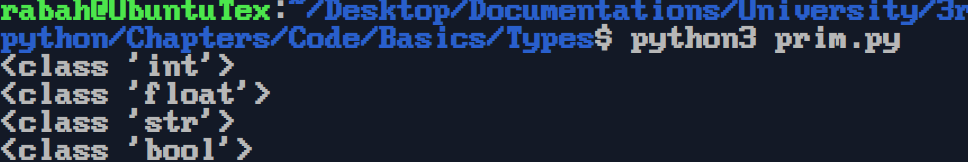
\includegraphics[width = 0.9\textwidth]{Chapters/ScreenShot/Basics/Types/primOutput.png}
\end{center}

\vspace{1cm}

\textbf{\underline{Non Primitive Example}}\\[0.1cm]
\lstinputlisting[style=pythonstyle]{Chapters/Code/Basics/Types/NonPrim.py}

\vspace{0.25cm}
\begin{center}
    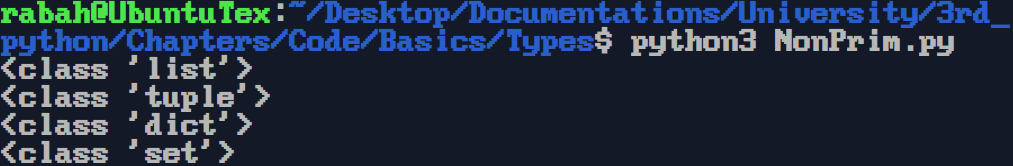
\includegraphics[width = 0.9\textwidth]{Chapters/ScreenShot/Basics/Types/NonPrimOutput.png}
\end{center}

\vspace{0.5cm}


\section{Comments}
\begin{prettyBox}{Comments}{myblue}
\begin{itemize}
    \item Single Line Comment : they start with \#
    \item Multi-Line Block Comment : wrapped between single or double quote : \texttt{'''} , \texttt{"""}
\end{itemize}
\end{prettyBox}

\vspace{0.35cm}
\textbf{\underline{Example}}\\[0.1cm]
\lstinputlisting[style=pythonstyle]{Chapters/Code/Basics/Comments/com.py}

\vspace{0.25cm}
\begin{center}
    
\includegraphics[width = 0.9\textwidth]{Chapters/ScreenShot/Basics/Comments/comOutput.png}
\end{center}

\vspace{1cm}
\section{Input/Output}
\begin{prettyBox}{IO}{myblue}
\begin{itemize}
    \item \texttt{print} : we use the print function to display text , 
        there are many string formatting we will see them in next section , the default formating
        is text between qout and we seprate variable with comma , and it automatically add space
    \item \texttt{input} : has message inside ,by default input takes in string variable.we can type
        cast it , we can input many var at once with split() , we use map when inputing many var + 
        typecasting
\end{itemize}
\end{prettyBox}

\vspace{0.5cm}
\textbf{\underline{Syntax}}\\[0.1cm]
\lstinputlisting[style=pythonstyle]{Chapters/Code/Basics/IO/syn.py}

\newpage
\textbf{\underline{Example}}\\[0.1cm]
\lstinputlisting[style=pythonstyle]{Chapters/Code/Basics/IO/io.py}


\vspace{0.25cm}
\begin{center}
    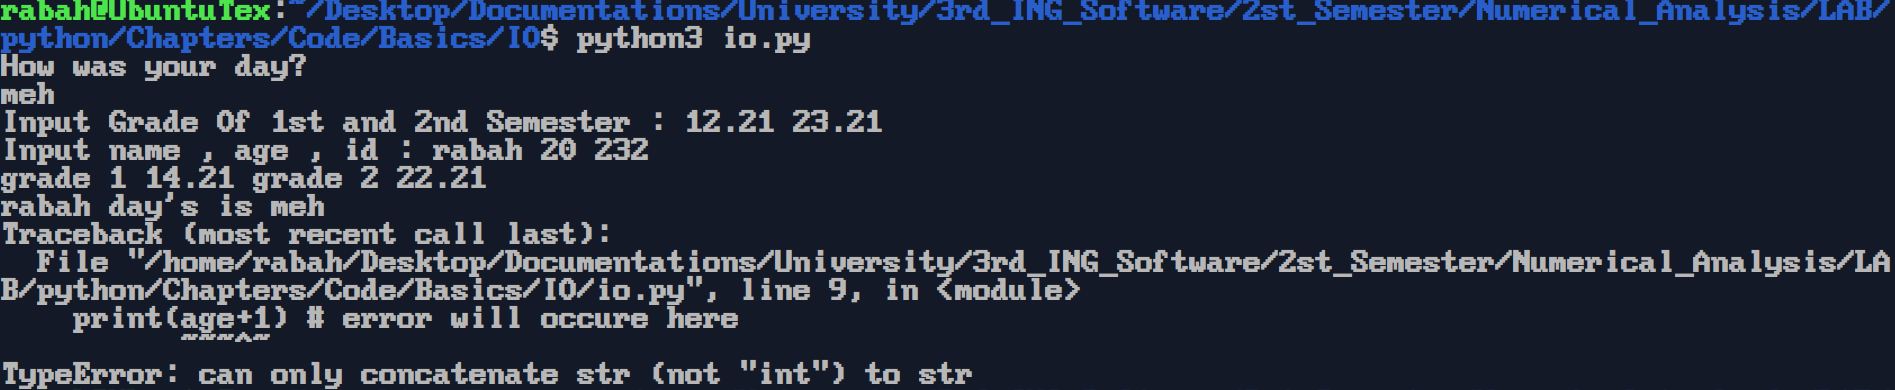
\includegraphics[width = 0.9\textwidth]{Chapters/ScreenShot/Basics/IO/ioOutput.png}
\end{center}

\vspace{1cm}
\section{String Formatting}

\begin{prettyBox}{Formatting}{myblue}
\begin{itemize}
    \item Default : Uses \texttt{print()} with values separated by commas, automatically adding spaces.
    \item f-string : Uses \texttt{f"\{var\}"}, treats \texttt{\textbackslash} as an escape character, and what's between \texttt{\{\}} is evaluated as a variable , Use \texttt{\{\{\}\}} for literal curly braces.
    \item raw-string : Uses \texttt{r"string"} to treat backslashes \texttt{\textbackslash} as literal characters.
    \item f+raw-string : Uses \texttt{fr"string"}, supports \texttt{\{var\}} formatting of f-string while treating \texttt{\textbackslash} as a literal character.
\item \% formatting : Uses \texttt{"format \% value"}, similar to C-style formatting.
    \item .format : Uses \texttt{"\{\} \{\}".format(val1, val2)} to insert values into placeholders. Placeholders can be empty, indexed, or labeled.
\end{itemize}
\end{prettyBox}

\vspace{0.5cm}

\newpage
\textbf{\underline{Example}}\\[0.1cm]
\lstinputlisting[style=pythonstyle]{Chapters/Code/Basics/Format/form.py}


\vspace{0.25cm}
\begin{center}
    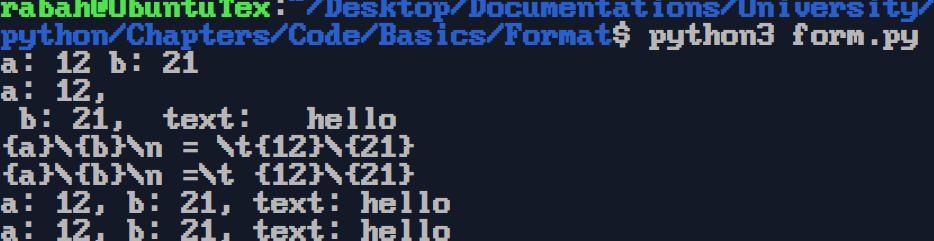
\includegraphics[width = 0.9\textwidth]{Chapters/ScreenShot/Basics/Format/formatOutput.png}
\end{center}

\vspace{1cm}

\section{Importing Modules}

\begin{prettyBox}{Import}{myblue}
A module in Python is simply a file containing Python code with classes , functions and variables that we can include and use in our own programs. There are two main ways to import modules:
\begin{itemize}
    \item \textbf{Importing the entire module}: This loads all the module’s functions, classes, and variables , to access them we need to
        write the modulename followed by a point
    \item \textbf{Importing specific parts of a module}: Instead of loading everything, we can import only specific functions, classes, or variables, which
        we call directly by their name.
\end{itemize}
\end{prettyBox}

\vspace{0.5cm}

\begin{prettyBox}{Note}{red}
\begin{itemize}
    \item We can rename imported modules or specific parts of a module using the \texttt{as} keyword.
    \item If we import multiple modules or module parts with the same name, Python will override previous imports with the latest one.
    \item One module can have submodules that can be accessed using . : \texttt{module.submodule}
\end{itemize}
\end{prettyBox}

\vspace{1cm}
\textbf{\underline{Syntax}}\\[0.1cm]
\lstinputlisting[style=pythonstyle]{Chapters/Code/Basics/Import/syn.py}


\vspace{0.8cm}

\textbf{\underline{Example}}\\[0.1cm]
\lstinputlisting[style=pythonstyle]{Chapters/Code/Basics/Import/im.py}


\vspace{0.35cm}
\begin{center}
    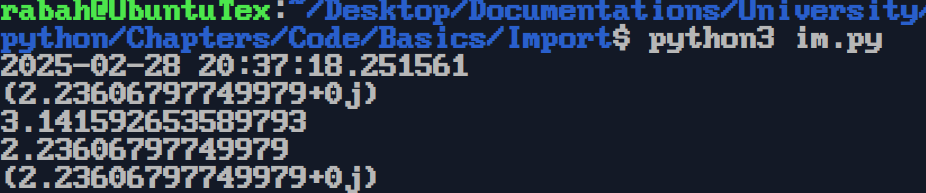
\includegraphics[width = 0.9\textwidth]{Chapters/ScreenShot/Basics/Import/imOutput.png}
\end{center}

\newpage


\section{Operators}
\begin{prettyBox}{Operators}{myblue}
\begin{itemize}
    \item \textbf{Arithmetic Operators}:
        \begin{itemize}
            \item \texttt{+} : Addition
            \item \texttt{-} : Subtraction
            \item \texttt{*} : Multiplication
            \item \texttt{/} :  Float division 
            \item \texttt{//} : Integer division 
            \item \texttt{\%} : Modulo 
            \item \texttt{**} : Exponentiation (power)
            \item \texttt{=} : Assignment 
        \end{itemize}
    
    \item \textbf{Comparison Operators}:
        \begin{itemize}
            \item \texttt{==} : Equal to 
            \item \texttt{!=} : Not equal to 
            \item \texttt{>} : Greater than
            \item \texttt{<} : Less than
            \item \texttt{>=} : Greater than or equal to
            \item \texttt{<=} : Less than or equal to
        \end{itemize}

    \item \textbf{Logical Operators}:
        \begin{itemize}
            \item \texttt{and} : Logical AND 
            \item \texttt{or} : Logical OR 
            \item \texttt{not} : Logical NOT 
        \end{itemize}
\end{itemize}
\end{prettyBox}

\newpage
\section{Control Structures}
\begin{prettyBox}{Control Structures}{myblue}
Python does not use curly braces (\{\}) to define control structures, classes, or functions.  
Instead, it relies on indentation to determine code blocks 4 spaces.In this section, we will explore all control structures with syntax and examples.
\end{prettyBox}

\vspace{1cm}
\subsection{If Statement}
\textbf{\underline{Syntax}}\\[0.1cm]
\lstinputlisting[style=pythonstyle]{Chapters/Code/Basics/Control/synif.py}


\vspace{0.8cm}

\textbf{\underline{Example}}\\[0.1cm]
\lstinputlisting[style=pythonstyle]{Chapters/Code/Basics/Control/if.py}

\vspace{0.35cm}
\begin{center}
    
\includegraphics[width = 0.9\textwidth]{Chapters/ScreenShot/Basics/Control/ifOutput.png}
\end{center}

\newpage
\subsection{Match Statement(Switch Case)}
\textbf{\underline{Syntax}}\\[0.1cm]
\lstinputlisting[style=pythonstyle]{Chapters/Code/Basics/Control/synswitch.py}


\vspace{0.8cm}

\textbf{\underline{Example}}\\[0.1cm]
\lstinputlisting[style=pythonstyle]{Chapters/Code/Basics/Control/switch.py}

\vspace{0.35cm}
\begin{center}
    
\includegraphics[width = 0.9\textwidth]{Chapters/ScreenShot/Basics/Control/switchOutput.png}
\end{center}

\newpage
\subsection{While Loop}
\textbf{\underline{Syntax}}\\[0.1cm]
\lstinputlisting[style=pythonstyle]{Chapters/Code/Basics/Control/synwhile.py}


\vspace{0.8cm}

\textbf{\underline{Example}}\\[0.1cm]
\lstinputlisting[style=pythonstyle]{Chapters/Code/Basics/Control/while.py}

\vspace{0.35cm}
\begin{center}
    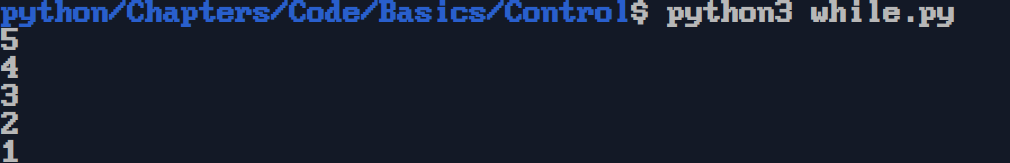
\includegraphics[width = 0.9\textwidth]{Chapters/ScreenShot/Basics/Control/whileOutput.png}
\end{center}

\vspace{1cm}
\subsection{For Loop}
\textbf{\underline{Syntax}}\\[0.1cm]
\lstinputlisting[style=pythonstyle]{Chapters/Code/Basics/Control/synfor.py}


\newpage

\textbf{\underline{Example}}\\[0.1cm]
\lstinputlisting[style=pythonstyle]{Chapters/Code/Basics/Control/for.py}

\vspace{0.35cm}
\begin{center}
    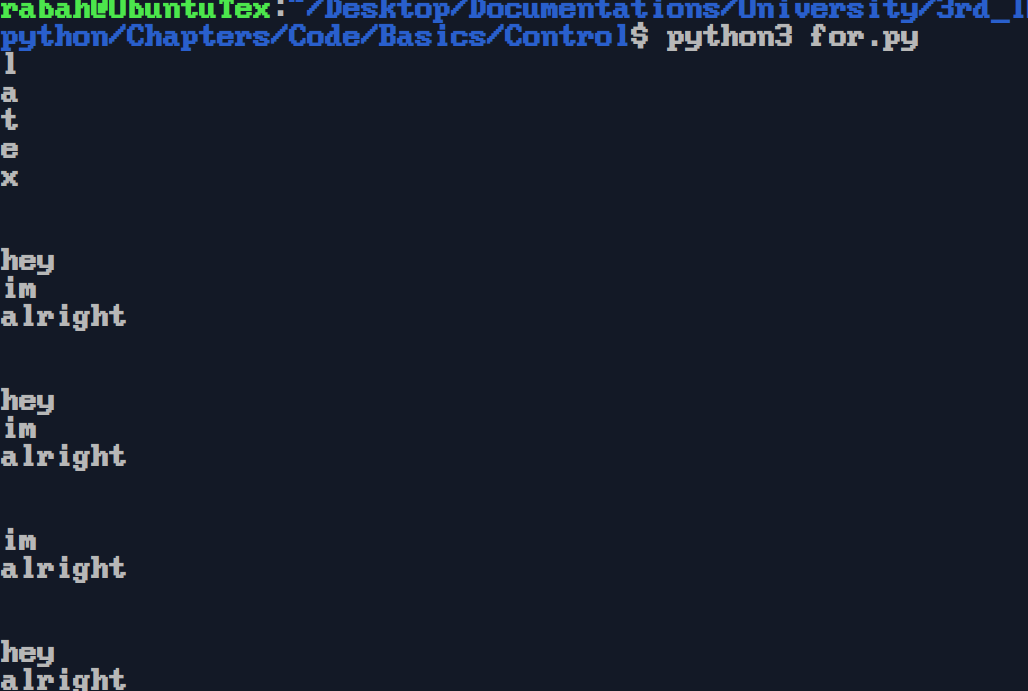
\includegraphics[height = 0.4\textheight]{Chapters/ScreenShot/Basics/Control/forOutput.png}
\end{center}

\newpage
\section{Function}
\textbf{\underline{Syntax}}\\[0.1cm]
\lstinputlisting[style=pythonstyle]{Chapters/Code/Basics/Function/synfunc.py}


\vspace{0.5cm}

\textbf{\underline{Example}}\\[0.1cm]
\lstinputlisting[style=pythonstyle]{Chapters/Code/Basics/Function/func.py}

\vspace{0.35cm}
\begin{center}
    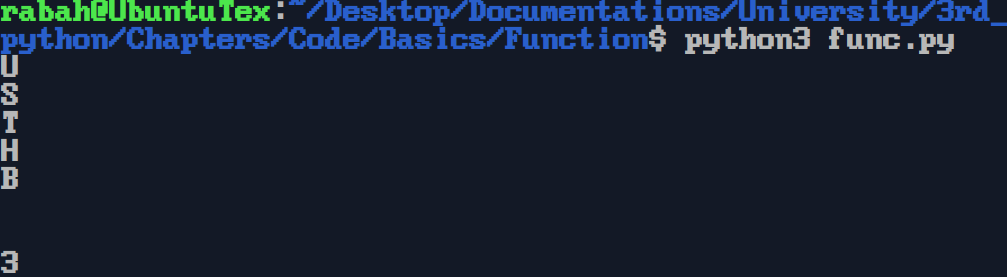
\includegraphics[width = 0.9\textwidth]{Chapters/ScreenShot/Basics/Function/funcOutput.png}
\end{center}

\newpage

\section{NamedTuple}
\begin{prettyBox}{NamedTuple}{myblue}
NamedTuples are similar to structures in C. The key difference is that they have the same properties as tuples, meaning their elements are immutable, so we cannot modify them directly only override them with new ones.\\[0.05cm]
To create a NamedTuples, we need to import the \texttt{namedtuple} function from the \texttt{collections} module. It takes the name of the tuple and its attributes as parameters.
\end{prettyBox}

\vspace{1cm}
\textbf{\underline{Syntax}}\\[0.1cm]
\lstinputlisting[style=pythonstyle]{Chapters/Code/Basics/Struct/synst.py}

\vspace{0.5cm}

\textbf{\underline{Example}}\\[0.1cm]
\lstinputlisting[style=pythonstyle]{Chapters/Code/Basics/Struct/st.py}

\vspace{0.35cm}
\begin{center}
    
\includegraphics[width = 0.9\textwidth]{Chapters/ScreenShot/Basics/Struct/stOutput.png}
\end{center}



\newpage
\begin{center}
    \Huge{\textbf{\underline{Chapter 2: NumPy}}}
\end{center}

\setcounter{section}{0}

\section{Introduction}
\begin{prettyBox}{Introduction}{myblue}
NumPy(Numerical Python) is a fundamental library for Python 
numerical computing. It provides efficient multi-dimensional 
array objects and various mathematical functions for handling 
large datasets.\\[0.1cm]
To use NumPy, we need to import the \texttt{numpy} module. By 
convention, it is commonly aliased as \texttt{np} to simplify usage 
and improve readability.
\end{prettyBox}

\vspace{0.5cm}

\section{Array}
\begin{prettyBox}{Array}{myblue}  
NumPy arrays are more efficient and faster than the collections we have seen so far. They 
allow operations to be performed on the entire array at once, eliminating the need for looping 
through elements individually. We can create NumPy arrays using built-in functions or convert 
existing lists into arrays using the \texttt{array} function.  
\end{prettyBox}

\vspace{0.5cm}
\subsection{Converting List To Array}
\begin{prettyBox}{Converting}{myblue}
To convert a list into an NumPy array we the \text{array()} function.
\end{prettyBox}

\vspace{1cm}
\textbf{\underline{Syntax}}\\[0.1cm]
\lstinputlisting[style=pythonstyle]{Chapters/Code/NP/Array/synar.py}

\vspace{0.5cm}

\textbf{\underline{Example}}\\[0.1cm]
\lstinputlisting[style=pythonstyle]{Chapters/Code/NP/Array/ar.py}


\subsection{Generating Arrays}
\begin{prettyBox}{Generating}{myblue}
\begin{itemize}
    \item \textbf{\texttt{arange(start=0, stop, step=1, dtype=None)}} : Creates an array of values 
    with a specified step size. 
    \begin{itemize}
        \item \textbf{start} (default = 0) is optional the beginning of the sequence.
        \item \textbf{stop} is the end value (not included in the array).
        \item \textbf{step} (default = 1) determines the increment.
        \item \textbf{dtype} is optional and defines the data type. If not specified, NumPy infers it automatically.
    \end{itemize}

    \item \textbf{\texttt{linspace(start, stop, num=50, endpoint=True, retstep=False, dtype=None, axis=0)}} : 
    Generates an array of num element evenly spaced values.
    \begin{itemize}
        \item \textbf{start} is the first value in the sequence.
        \item \textbf{stop} is the last value (included by default if \texttt{endpoint=True}).
        \item \textbf{num} (default = 50) specifies the total number of values.
        \item \textbf{endpoint} is optional (default = True) determines whether \texttt{stop} is included.
        \item \textbf{retstep} is optional (default = False) returns the step size if set to True.
        \item \textbf{dtype} is optional and specifies the data type.
        \item \textbf{axis} is optional (default = 0) is used in multi-dimensional arrays.
    \end{itemize}
\end{itemize}
\end{prettyBox}

\vspace{1cm}
\textbf{\underline{Arange()}}\\[0.05cm]
\textbf{\underline{Syntax}}\\[0.1cm]
\lstinputlisting[style=pythonstyle]{Chapters/Code/NP/Array/sysar.py}

\vspace{0.5cm}

\textbf{\underline{Example}}\\[0.1cm]
\lstinputlisting[style=pythonstyle]{Chapters/Code/NP/Array/arr.py}

\newpage

\vspace{0.25cm}
\begin{center}
    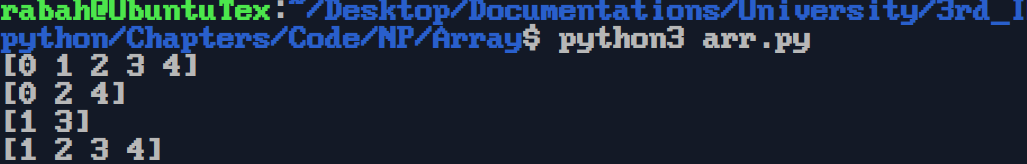
\includegraphics[width = 0.9\textwidth]{Chapters/ScreenShot/NP/Array/arOutput.png}
\end{center}

\vspace{1cm}



\textbf{\underline{LinSpace()}}\\[0.05cm]
\textbf{\underline{Syntax}}\\[0.1cm]
\lstinputlisting[style=pythonstyle]{Chapters/Code/NP/Array/syslin.py}

\vspace{0.5cm}

\textbf{\underline{Example}}\\[0.1cm]
\lstinputlisting[style=pythonstyle]{Chapters/Code/NP/Array/lin.py}

\vspace{0.25cm}
\begin{center}
    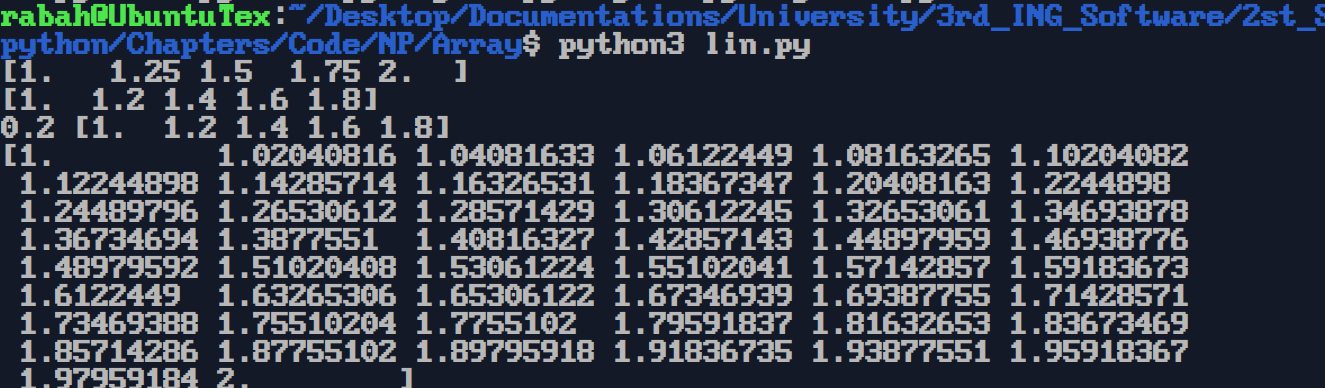
\includegraphics[width = 0.9\textwidth]{Chapters/ScreenShot/NP/Array/linOutput.png}
\end{center}

\vspace{1cm}

\subsection{Array Slicing}
\begin{prettyBox}{Slicing}{myblue}
\texttt{array[start=0 : stop=len(array) : step=1]}
\begin{itemize}
    \item \textbf{start} (default = 0): The index where slicing begins. If negative, it is interpreted as \texttt{len(array) + start}.
    \item \textbf{stop} (default = \texttt{len(array)}): The index where slicing ends (exclusive). If negative, it is interpreted as \texttt{len(array) + stop}.
    \item \textbf{step} (default = 1): Determines the stride between elements. Can be negative for reverse slicing.
\end{itemize}
\end{prettyBox}

\vspace{0.5cm}

\textbf{\underline{Example}}\\[0.1cm]
\lstinputlisting[style=pythonstyle]{Chapters/Code/NP/Array/slice.py}

\vspace{0.25cm}
\begin{center}
    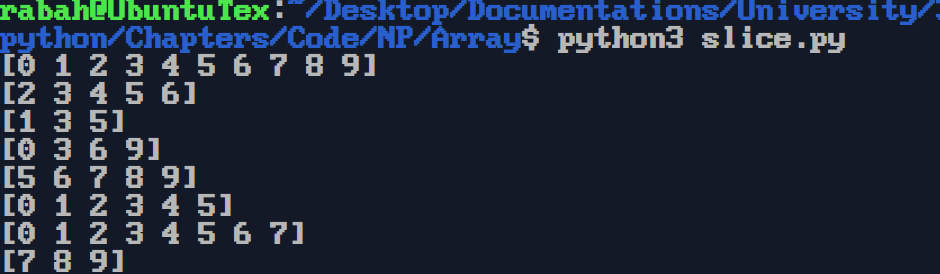
\includegraphics[width = 0.9\textwidth]{Chapters/ScreenShot/NP/Array/sliceOutput.png}
\end{center}

\newpage
\section{Mathematical Function}
\begin{prettyBox}{Function}{myblue}
\begin{itemize}
    \item \texttt{sin(x)} : \(\sin{(x)}\)  
    \item \texttt{cos(x)} : \(\cos{(x)}\)
    \item \texttt{tan(x)} : \(\tan{(x)}\)
    \item \texttt{exp(x)} : \(e^{x}\)
    \item \texttt{log(x)} : \(\ln{(x)}\) 
    \item \texttt{log10(x)} : \(\log_{10}{(x)}\)
    \item \texttt{log2(x)} : \(\log_{2}{(x)}\)
    \item \texttt{log(x) / log(b)} : \(\log_b{(x)}\)
\end{itemize}
\end{prettyBox}

\newpage
\begin{center}
    \Huge{\textbf{\underline{Chapter 3: MatPlotLib}}}
\end{center}

\setcounter{section}{0}


\section{Introduction}
\begin{prettyBox}{Introduction}{myblue}
Matplotlib is a powerful Python library for data visualization. It allows users to create both
static and interactive plots with ease. \\[0.1cm]
To use Matplotlib, we import the \texttt{pyplot} submodule, which provides a simple interface
for plotting. By convention, it is commonly aliased as \texttt{plt} to enhance readability and
simplify usage.
\end{prettyBox}

\vspace{0.5cm}


\section{Figure \& Axis}
\begin{prettyBox}{Difference}{myblue}
A \textbf{Figure} is the top-level container that holds everything, similar to a window or a canvas.  
An \textbf{Axis} is a plotting area inside a Figure where data is drawn.  

A single Figure can contain multiple Axes (subplots), allowing multiple plots within the same window.
\end{prettyBox}

\vspace{0.5cm}

\begin{center}
    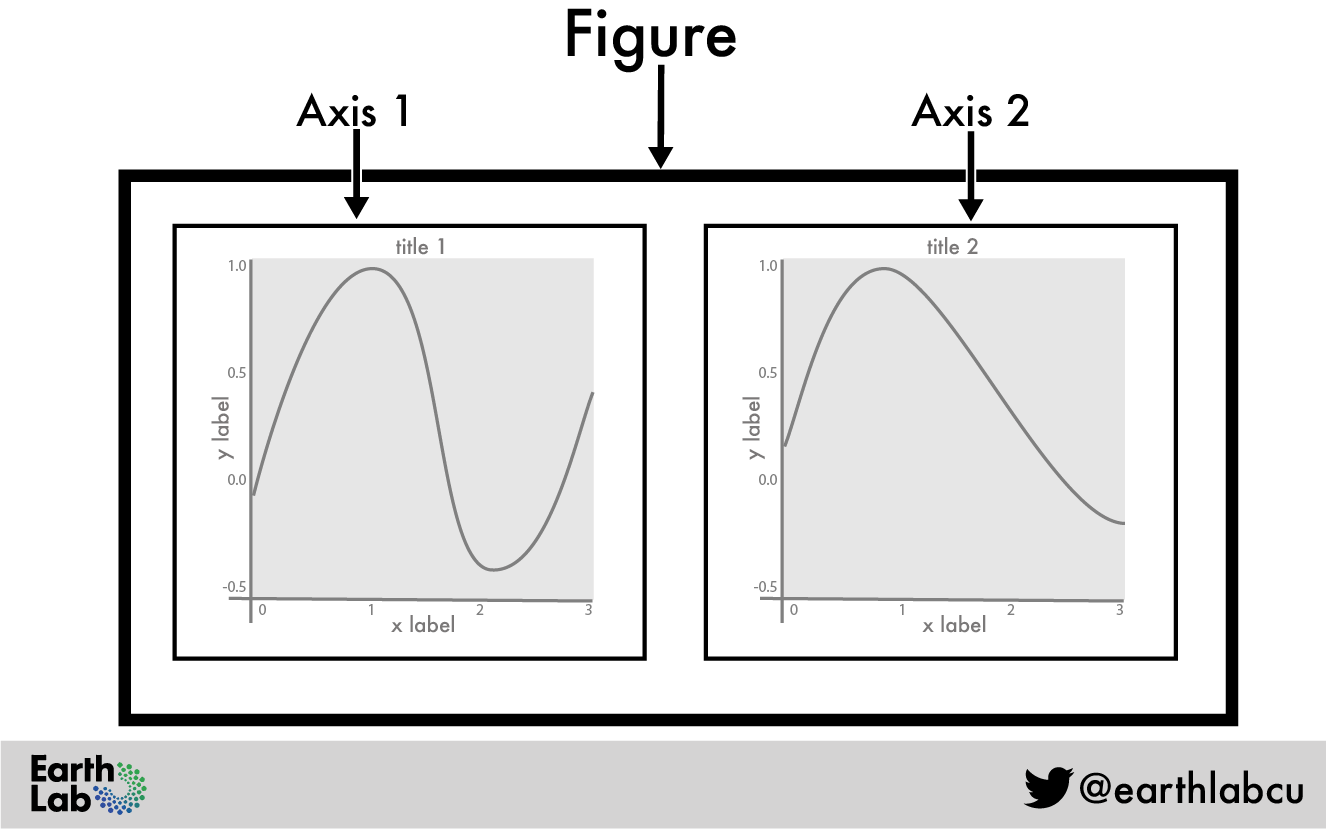
\includegraphics[height = 0.4\textheight]{Chapters/PNG/figureAxis.png}
\end{center}


\section{Creating a Figure}
\begin{prettyBox}{Figure Creation}{myblue}
\begin{itemize}
    \item A figure is created using the \texttt{figure()} function from the \texttt{pyplot} submodule.
    \item By default, Matplotlib starts with an implicit figure.
    \item Each additional call to \texttt{figure()} creates a new figure, so the total number of figures is :
        \begin{center}
            \boxed{\texttt{1 + (number of calls to figure())}}
        \end{center}
\end{itemize}
\end{prettyBox}

\vspace{0.5cm}


\section{Drawing A Plot}
\begin{prettyBox}{Plot}{myblue}
\texttt{plot()} is a function from the \texttt{pyplot} submodule used to draw a graph on the axis of a figure.\\[0.05cm] 
\texttt{plot(x, y, linestyle='-', linewidth=1.5, marker=None, markersize=6.0, color=auto, mfc=color, mec=color, label=None, alpha=1)}

\begin{itemize}
    \item \textbf{x}: A NumPy array representing the x-coordinates of the data points.
    \item \textbf{y}: A NumPy array representing the y-coordinates of the data points.
    \item \textbf{linestyle}: Optional parameter. Default is \texttt{'-'}. Specifies the style of the connecting line.
    \item \textbf{linewidth}: Optional parameter. Default is \texttt{1.5}. Controls the thickness of the line.
    \item \textbf{marker}: Optional parameter. Default is \texttt{None}. Defines the shape of markers placed at data points.
    \item \textbf{markersize}: Optional parameter. Default is \texttt{6.0}. Sets the size of the markers.
    \item \textbf{color}: Optional parameter. Default is \texttt{auto}. If not set, Matplotlib assigns a color automatically. Accepts color names, hex codes, and RGB(A) tuples.
    \item \textbf{mfc} (Marker Face Color): Optional parameter. Default is the same as \texttt{color}. Defines the fill color of the marker.
    \item \textbf{mec} (Marker Edge Color): Optional parameter. Default is the same as \texttt{color}. Defines the outline color of the marker.
    \item \textbf{label}: Optional parameter. Default is \texttt{None}. Specifies the legend label for the plot. Supports raw strings and LaTeX expressions using \texttt{\$ \$}.
    \item \textbf{alpha}: Optional parameter. Default is \texttt{1}. Controls the transparency of both lines and markers (1 = fully opaque, 0 = fully transparent).
\end{itemize}
\end{prettyBox}

\newpage

\begin{center}
    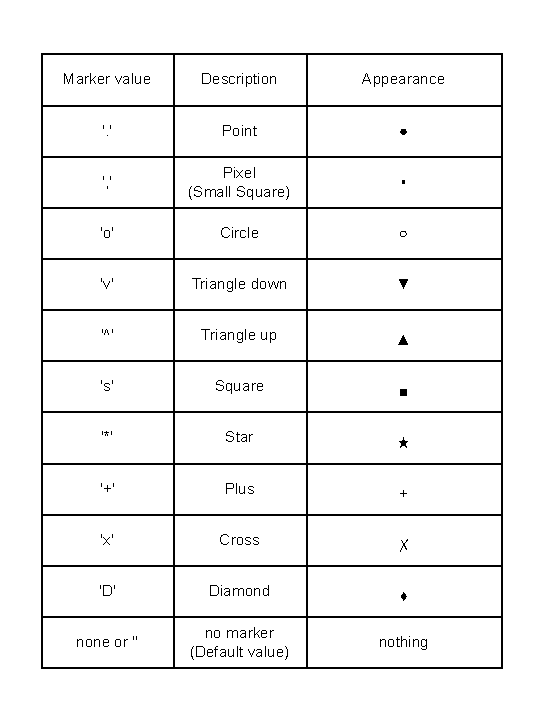
\includegraphics[height=0.6\textheight]{Chapters/PDF/marker.drawio.pdf}
\end{center}

\begin{center}
    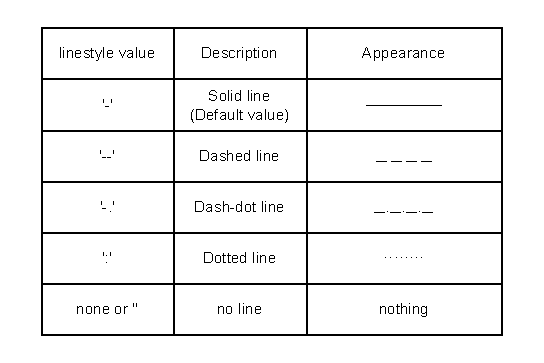
\includegraphics[height=0.35\textheight]{Chapters/PDF/linestyle.drawio.pdf}
\end{center}

\newpage

\section{Drawing a Single Point}
\begin{prettyBox}{Single Point}{myblue}
We can use either the \texttt{plot()} or \texttt{scatter()} function:
\begin{itemize}
    \item \texttt{plot(x, y, color=auto,linestyle='', marker, mfc=color, mec=color, alpha=1)}
    \item \texttt{scatter(x, y, color=auto, marker, c=color, edgecolors=color, alpha=1)}  
          Here, \texttt{c} is equivalent to \texttt{mfc}, and \texttt{edgecolors} is equivalent to \texttt{mec}.
\end{itemize}
\end{prettyBox}

\vspace{0.5cm}

\section{Graph Customization \& Display}
\begin{prettyBox}{Customization}{myblue}
\begin{itemize}
    \item \texttt{legend()}: Displays the labels of plotted elements (e.g., lines, scatter points) as a legend for the axis.
    \item \texttt{grid(visible=True)}: Toggles the grid on the axis. By default, the grid is off, but calling the function without arguments is equivalent to setting it to \texttt{True}.
    \item \texttt{title(label)}: Sets the title for the current axis.
    \item \texttt{suptitle(label)}: Sets the title for the current figure.
    \item \texttt{ylabel(label)}: Labels the y-axis.
    \item \texttt{xlabel(label)}: Labels the x-axis.
    \item \texttt{show()}: Renders and displays all created figures along with their content.
    \item \texttt{plt.savefig(fname)}: saves the figure in the given path fname , if fname doesn't have a file extension it will save it as png
\end{itemize}
\end{prettyBox}

\vspace{0.5cm}

\section{Subplot}
\begin{prettyBox}{Subplot}{myblue}
The \texttt{subplot()} function allows us to create multiple axes within the same figure by defining a grid layout.  

\texttt{subplot(nrows, ncols, index)}

\begin{itemize}
    \item \textbf{nrows}: Number of rows in the subplot grid.
    \item \textbf{ncols}: Number of columns in the subplot grid.
    \item \textbf{index}: The position of the subplot, starting from 1 (left to right, top to bottom).
\end{itemize}

Each call to \texttt{subplot()} activates a different subplot within the figure.  
\end{prettyBox}

\newpage
\textbf{\underline{Example}}\\[0.1cm]
\lstinputlisting[style=pythonstyle]{Chapters/Code/PLT/figure.py}

\newpage
\textbf{\underline{fig1}}\\[0.1cm]
\begin{center}
    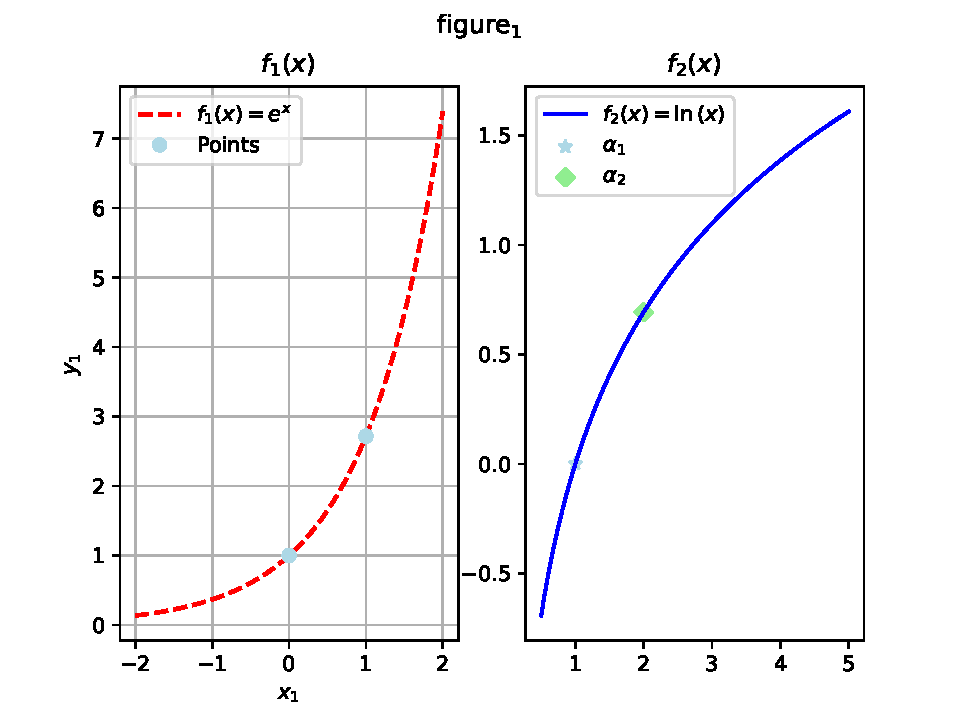
\includegraphics[height=0.35\textheight]{Chapters/Code/PLT/fig1.pdf}
\end{center}


\textbf{\underline{fig 2}}\\[0.1cm]
\begin{center}
    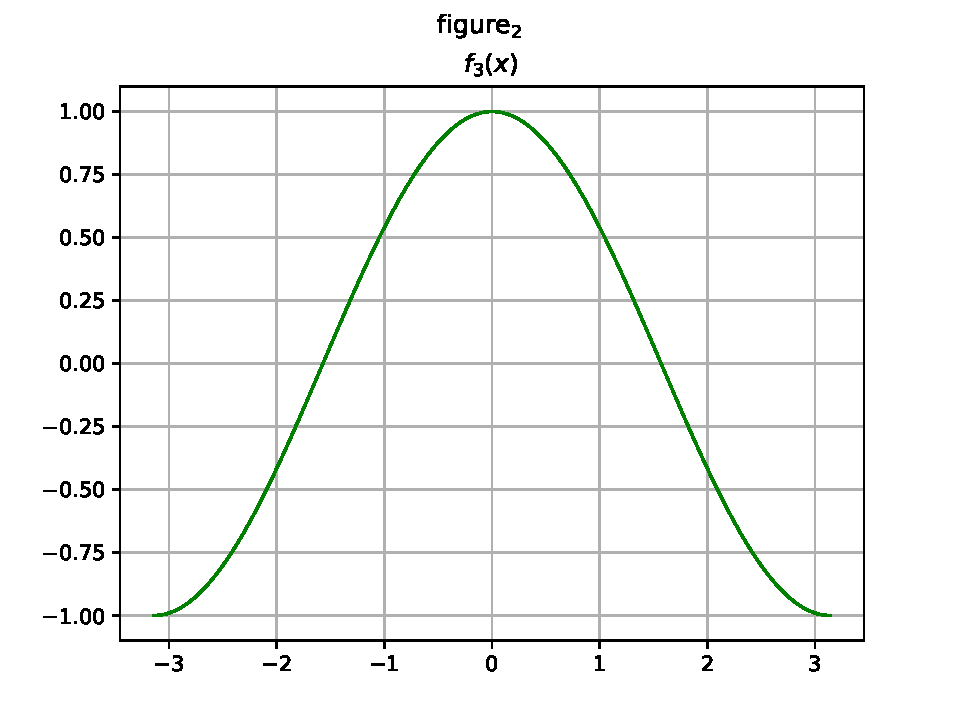
\includegraphics[height=0.35\textheight]{Chapters/Code/PLT/fig2.pdf}
\end{center}

\newpage

\begin{prettyBox}{Note}{red}
We can remove the \(x , y\) axes of an axis from showing by using the \texttt{plt.axis('off')} function.
\end{prettyBox}

\vspace{1cm}

\section{Drawing Tables}
\begin{prettyBox}{Table}{myblue}
To draw a table on an axis, we use the \texttt{table()} function, which returns a \texttt{Table} object.\\[0.1cm]
\texttt{the\_table = table(cellText, colLabels=None, rowLabels=None, cellLoc='right', fontsize=auto, colWidths=None, loc='bottom')}
\begin{itemize}
    \item \textbf{cellText}: A 2D list of strings that holds the content of each cell.
    \item \textbf{colLabels} (optional, default: \texttt{None}): A list of strings for the column headers.
    \item \textbf{rowLabels} (optional, default: \texttt{None}): A list of strings for the row headers.
    \item \textbf{cellLoc} (optional, default: \texttt{'right'}): Alignment of cell content. Possible values: \texttt{'right'}, \texttt{'left'}, \texttt{'center'}.
    \item \textbf{fontsize} (optional, default: \texttt{auto}): The font size of the table text.
    \item \textbf{colWidths} (optional): A list of floats representing the width of each column.
    \item \textbf{loc} (optional, default: \texttt{'bottom'}): The position of the table relative to the axes.
\end{itemize}

\vspace{0.15cm}

Some Function of \texttt{Table} object

\begin{itemize}
    \item \texttt{the\_table.auto\_set\_column\_width(col=None)} :  
        Adjusts the width of selected columns to fit their content.  
        \begin{itemize}
            \item \textbf{col} (optional, default: \texttt{None}): A list of integers representing the column indices to adjust.
        \end{itemize}

    \item \texttt{the\_table.scale(xscale, yscale)} :  
        Scales the table by adjusting cell padding.  
        \begin{itemize}
            \item \textbf{xscale} : Horizontal scaling factor.
            \item \textbf{yscale} : Vertical scaling factor.
        \end{itemize}

    \item \texttt{the\_table.auto\_set\_font\_size(scale=True)} :  
        Shrink font size until text fit in cell note that scaling padding with scale or calling the auto set columns width might override the behaviour
        of this function since text will always fit, and this behaviour is on by default.  
\begin{itemize}
    \item \textbf{scale} (optional , default = True) : boolean either True or False.
\end{itemize}

    \item \texttt{the\_table.set\_fontsize(size)} :  
        Manually sets the font size of the table text.
    \begin{itemize}
        \item \textbf{size} : float value. 
    \end{itemize}
   \end{itemize}
\end{prettyBox}

\newpage
\textbf{\underline{Example}}\\[0.1cm]
\lstinputlisting[style=pythonstyle]{Chapters/Code/PLT/tab.py}

\vspace{0.5cm}
\textbf{\underline{fig1}}\\[0.1cm]
\begin{center}
    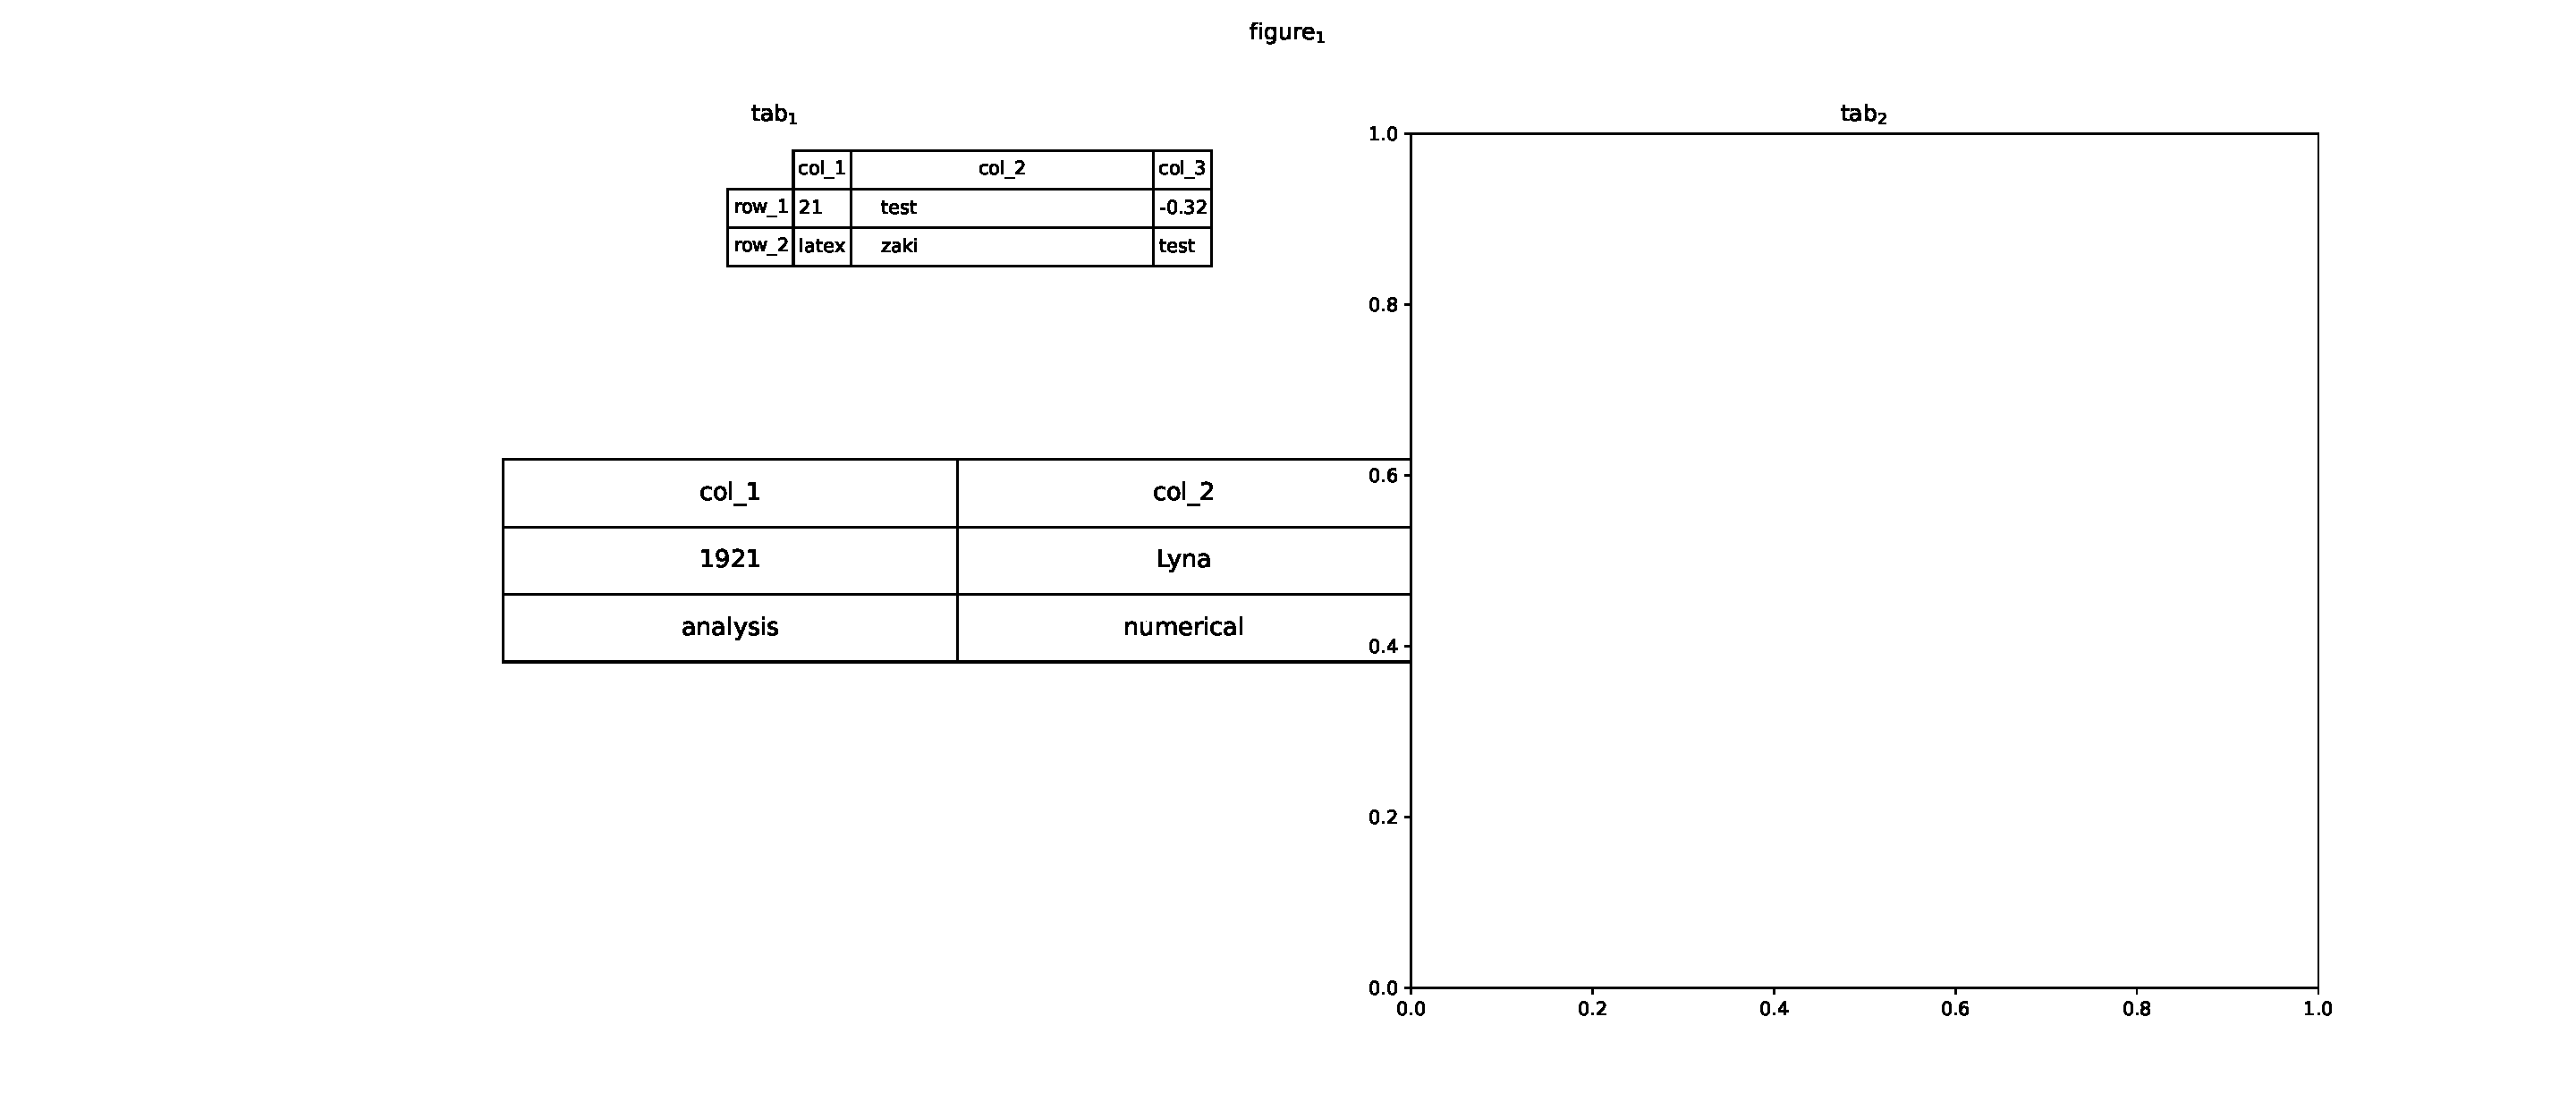
\includegraphics[height=0.35\textheight]{Chapters/Code/PLT/tab.pdf}
\end{center}




\newpage
\begin{center}
    \Huge{\textbf{\underline{Chapter 4: Dichotomy Mehtod}}}
\end{center}

\vspace{0.77cm}
\setcounter{section}{0}

\begin{prettyBox}{Implementation}{myblue}
\begin{itemize}
    \item \texttt{function(x)}: Returns the value of the function \( f(x) \) at a given point \( x \).
    \item \texttt{ErrorEstimation(a, b)}: Estimates the error for the interval \([a_n, b_n]\), where \( n \geq 0 \) : \(\dfrac{b_n-a_n}{2}\).
    \item \texttt{eps}: Represents the error tolerance \( \epsilon \).
    \item \texttt{max\_iter}: Specifies the maximum number of iterations for the while loop.
    \item \texttt{dichotomy(eps, a, b, function,max\_iter=100)}: Computes the root of the function \( f(x) \) using the dichotomy method over the interval \([a, b]\), with a given tolerance \( \epsilon \) ,
        and max number of iteration (100 by default).
\end{itemize}
\end{prettyBox}

\vspace{1cm}
\textbf{\underline{Code}}\\[0.1cm]
\lstinputlisting[style=pythonstyle]{Chapters/Code/DIC/dic.py}

\newpage
\textbf{\underline{Example}}\\[0.1cm]
\lstinputlisting[style=pythonstyle]{Chapters/Code/DIC/ex1.py}

\vspace{0.5cm}

\begin{center}
    
\includegraphics[width = 0.9\textwidth]{Chapters/ScreenShot/DIC/dic.png}
\end{center}


\newpage
\begin{center}
    \Huge{\textbf{\underline{Chapter 5: Fixed-Point Mehtod}}}
\end{center}

\vspace{0.77cm}
\setcounter{section}{0}

\begin{prettyBox}{Implementation}{myblue}
\begin{itemize}
\item \texttt{phi\_function(x)}: Computes the value of the function \( \varphi(x) \) at a
given point \( x_n \), following the recurrence relation:  
          \[
          x_{n+1} = \varphi(x_n)
          \]
\item \texttt{ErrorEstimation(a, b)}: Estimates the error at iteration \(n\) for a given 
contraction factor \( k \in ]0,1[\), using the formula:  
          \[
          \dfrac{k^n}{1-k} \cdot |x_0 - x_1|
          \]

    \item \texttt{eps}: Defines the error tolerance \( \epsilon \), determining the stopping
    criterion.

    \item \texttt{max\_iter}: Specifies the maximum number of iterations allowed in the 
fixed-point algorithm.

\item \texttt{Fixed\_Point(eps, k, x\_0, function, max\_iter=100)}: Computes the root of \( f(x) \) with the fixed-point method with the  
its corresponding \( \varphi(x) \) and contraction factor \( k \), starting from an
initial \( x_0 \) with a tolerance \( \epsilon \) and the maximum number of iterations max\_iter (default: 100).
\end{itemize}
\end{prettyBox}
\vspace{0.5cm}
\textbf{\underline{Code}}\\[0.05cm]
\lstinputlisting[style=pythonstyle]{Chapters/Code/FIX/fix.py}

\newpage
\textbf{\underline{Example}}\\[0.1cm]
\lstinputlisting[style=pythonstyle]{Chapters/Code/FIX/ex1.py}

\vspace{0.5cm}

\begin{center}
    
\includegraphics[width = 0.9\textwidth]{Chapters/ScreenShot/FIX/fix.png}
\end{center}


\end{document}
